\title[Measurement at high frequency]{Measurement and characterisation at high frequency}
\section{Measurement at high frequency}

\begin{frame}[plain]
	\titlepage
\end{frame}

%%%%%%%%%%%%%%%%%%%%%%%%%%%%%%%%%%%%%%%%%%%%%%%%%%%%%%%%%%%%%
%% Overview %%
%%%%%%%%%%%%%%%%%%%%%%%%%%%%%%%%%%%%%%%%%%%%%%%%%%%%%%%%%%%%%
\subsection{Measurement chain}

\begin{frame}
	\frametitle{Overview}
	A GaN half-bridge switches 48\,V in about 1\,ns and rings at several hundred MHz. Every probe, wire and sensor that we connect becomes part of the circuit, and every nanosecond of delay between two channels changes the measured loss.
	\begin{itemize}
		\item Bandwidth, rise time, probe loading and the ground lead
		\item Voltage probes and current sensors for fast edges; deskew
		\item Device characterisation: double-pulse test, $C_\mathrm{oss}$ loss, dynamic $R_\mathrm{DS(on)}$
		\item Impedance of capacitors and magnetic components; core loss at MHz
		\item Efficiency and temperature: how large is the error?
	\end{itemize}
	After this lecture you can choose a measurement set-up for a MHz converter, estimate its error and recognise measurement artefacts.
\end{frame}

%%%%%%%%%%%%%%%%%%%%%%%%%%%%%%%%%%%%%%%%%%%%%%%%%%%%%%%%%%%%%
%% Bandwidth and rise time %%
%%%%%%%%%%%%%%%%%%%%%%%%%%%%%%%%%%%%%%%%%%%%%%%%%%%%%%%%%%%%%
\begin{frame}
	\frametitle{Bandwidth and rise time}
	\begin{columns}[T]
		\begin{column}{0.5\textwidth}
			\begin{figure}
				\centering
				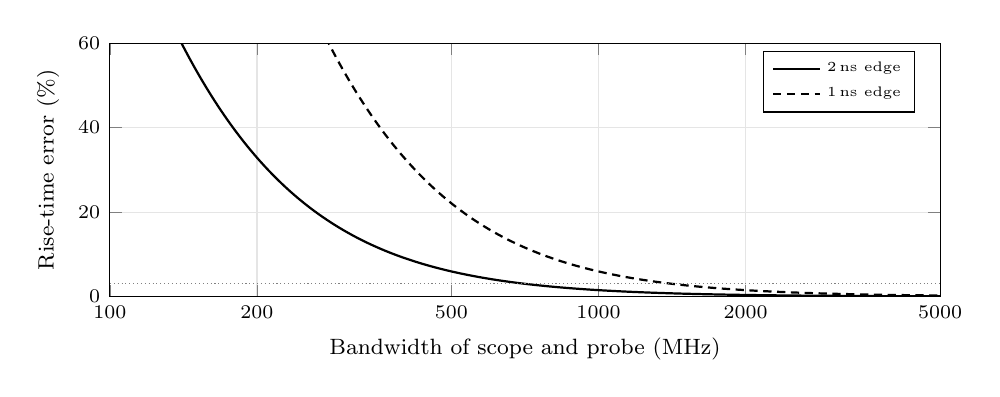
\begin{tikzpicture}
					\begin{axis}[
							width=\linewidth, height=4.8cm,
							xmode=log, xmin=100, xmax=5000, ymin=0, ymax=60,
							xtick={100,200,500,1000,2000,5000}, xticklabels={100,200,500,1000,2000,5000},
							xlabel={Bandwidth of scope and probe (MHz)}, ylabel={Rise-time error (\%)},
							grid=major, grid style={gray!20},
							tick label style={font=\scriptsize}, label style={font=\footnotesize},
							legend style={font=\tiny}, legend pos=north east, legend cell align=left,
						]
						\addplot[black, thick, domain=100:5000, samples=200] {(sqrt(1+(0.35/(x*1e6*2e-9))^2)-1)*100};
						\addlegendentry{2\,ns edge}
						\addplot[black, thick, densely dashed, domain=100:5000, samples=200] {(sqrt(1+(0.35/(x*1e6*1e-9))^2)-1)*100};
						\addlegendentry{1\,ns edge}
						\addplot[gray, densely dotted, domain=100:5000, samples=2] {3};
					\end{axis}
				\end{tikzpicture}
				\caption{Error of the measured 10--90\,\% rise time, Gaussian response; dotted: 3\,\%}
			\end{figure}
		\end{column}
		\begin{column}{0.47\textwidth}
			\small
			\begin{itemize}
				\item $t_\mathrm{r}\approx0.35/f_\mathrm{BW}$ for a Gaussian response, about $0.4/f_\mathrm{BW}$ for a maximally flat one (scopes above 1\,GHz).
				\item Rise times add geometrically:
				      \begin{equation*}
					      t_\mathrm{r,meas}=\sqrt{t_\mathrm{r,sig}^2+t_\mathrm{r,probe}^2+t_\mathrm{r,scope}^2}
				      \end{equation*}
				\item For 3\,\% error the chain must be four times faster than the signal: 1\,ns needs about 1.4\,GHz.
				\item An edge contains frequencies up to $f_\mathrm{knee}\approx0.5/t_\mathrm{r}$. EPC2045 needs 0.5--1\,GHz, the smallest GaN dies more.
			\end{itemize}
		\end{column}
	\end{columns}
	\blfootnote{Sources: Keysight, Evaluating Oscilloscope Bandwidths for Your Application, 5989-5733EN, 2019; Lidow et al., 2019, Sec.\ 5.3.1 and Tab.\ 5.3.}
\end{frame}

%%%%%%%%%%%%%%%%%%%%%%%%%%%%%%%%%%%%%%%%%%%%%%%%%%%%%%%%%%%%%
%% Your turn: rise time %%
%%%%%%%%%%%%%%%%%%%%%%%%%%%%%%%%%%%%%%%%%%%%%%%%%%%%%%%%%%%%%
% Two pages: task (page 1) and task with solution (page 2).
\begin{frame}<handout:1-2>
	\frametitle{Rise-time error}
	\begin{block}{Task (3 minutes)}
		The switch-node voltage of a GaN half-bridge rises in 2\,ns. It is measured with a 350\,MHz oscilloscope and a 500\,MHz probe.
		\begin{enumerate}
			\item Which rise time does the scope show?
			\item Which bandwidth of scope and probe is needed for an error below 3\,\%?
		\end{enumerate}
	\end{block}
	\onslide<2-|handout:2>{
		\begin{enumerate}
			\item $t_\mathrm{r,scope}=0.35/350\,\mathrm{MHz}=1.0$\,ns, $t_\mathrm{r,probe}=0.35/500\,\mathrm{MHz}=0.7$\,ns:
			      \begin{equation*}
				      t_\mathrm{r,meas}=\sqrt{2^2+1^2+0.7^2}\,\mathrm{ns}=2.34\,\mathrm{ns}\quad(+17\,\%)
			      \end{equation*}
			      The edge appears slower, and $\mathrm{d}v/\mathrm{d}t$ and the overshoot appear smaller.
			\item The chain may have at most $0.25\,t_\mathrm{r,sig}=0.5$\,ns: $f_\mathrm{BW}\geq0.35/0.5\,\mathrm{ns}=0.7$\,GHz for scope and probe together, i.e.\ about 1\,GHz each.
		\end{enumerate}
	}
\end{frame}

%%%%%%%%%%%%%%%%%%%%%%%%%%%%%%%%%%%%%%%%%%%%%%%%%%%%%%%%%%%%%
%% Probe loading and ground lead %%
%%%%%%%%%%%%%%%%%%%%%%%%%%%%%%%%%%%%%%%%%%%%%%%%%%%%%%%%%%%%%
\begin{frame}
	\frametitle{Probe loading and ground lead}
	\begin{columns}[T]
		\begin{column}{0.42\textwidth}
			\begin{figure}
				\centering
				\begin{circuitikz}[scale=0.75, transform shape]
					\draw (0,0) node[ground]{} to[sV, l=$v_\mathrm{sw}$] (0,2.8) -- (1.0,2.8) node[circ]{} node[above]{tip};
					\draw (1.0,2.8) -- (3.4,2.8) to[R, l=$R_\mathrm{p}$] (3.4,1.4) coordinate (a);
					\draw (a) -- (5.7,1.4) to[C, l=$C_\mathrm{p}$] (5.7,0) coordinate (b);
					\draw (a) to[R, l=10\,M$\Omega$] (3.4,0) -- (b);
					\draw (3.4,0) -- (3.0,0) to[L, l=$L_\mathrm{g}$] (1.0,0) -- (0,0);
					\draw[densely dashed, gray] (2.95,-0.45) rectangle (6.9,3.2);
					\node[font=\scriptsize, anchor=south] at (4.9,3.2) {probe};
					\node[font=\scriptsize, anchor=north] at (2.0,-0.75) {ground lead};
				\end{circuitikz}
				\caption{Passive probe with ground lead (simplified)}
			\end{figure}
		\end{column}
		\begin{column}{0.55\textwidth}
			\small
			\begin{itemize}
				\item A 10:1 passive probe has a few pF: 4\,pF is 400\,$\Omega$ at 100\,MHz. Negligible at the switch node, not at a gate or sense node.
				\item The ground lead adds about 1\,nH per mm. With 160\,mm and 4\,pF it resonates at $f_\mathrm{p}=1/(2\pi\sqrt{L_\mathrm{g}C_\mathrm{p}})=200$\,MHz. Every fast edge excites this resonance: the scope shows ringing that does not exist.
				\item Spring tip or ground spring (a few mm, a few nH): $f_\mathrm{p}$ above 1\,GHz.
				\item The ground loop also picks up the field of the power loop.
			\end{itemize}
		\end{column}
	\end{columns}
	\blfootnote{Sources: ROHM, Method for Monitoring Switching Waveform, application note; Lidow et al., 2019, Sec.\ 5.3.2.}
\end{frame}

%%%%%%%%%%%%%%%%%%%%%%%%%%%%%%%%%%%%%%%%%%%%%%%%%%%%%%%%%%%%%
%% Spot the artefact %%
%%%%%%%%%%%%%%%%%%%%%%%%%%%%%%%%%%%%%%%%%%%%%%%%%%%%%%%%%%%%%
% Two pages: question (page 1) and answer (page 2).
\begin{frame}<handout:1-2>
	\frametitle{Spot the artefact}
	\begin{columns}[T]
		\begin{column}{0.55\textwidth}
			\begin{figure}
				\centering
				\begin{tikzpicture}
					\begin{axis}[
							width=\linewidth, height=5.0cm,
							xmin=-1, xmax=20, ymin=-5, ymax=130,
							xlabel={Time (ns)}, ylabel={Measured $v_\mathrm{sw}$ (V)},
							grid=major, grid style={gray!20},
							tick label style={font=\scriptsize}, label style={font=\footnotesize},
							legend style={font=\tiny}, legend pos=north east, legend cell align=left,
						]
						\addplot[gray, thick] table[x=t, y=clip] {fig/lec05/probe_artefact.dat};
						\addlegendentry{probe A}
						\addplot[black, thick] table[x=t, y=spring] {fig/lec05/probe_artefact.dat};
						\addlegendentry{probe B}
					\end{axis}
				\end{tikzpicture}
				\caption{The same 48\,V switch-node edge, measured twice with a 500\,MHz scope}
			\end{figure}
		\end{column}
		\begin{column}{0.42\textwidth}
			\small
			Probe A shows 123\,V and rings at 200\,MHz, probe B shows 80\,V and rings at 300\,MHz. The power loop has 1\,nH, the switch node 280\,pF.\\[0.4em]
			Which waveform is real? Vote.
			\onslide<2-|handout:2>{
				\begin{block}{Answer: B}
					$1/(2\pi\sqrt{1\,\mathrm{nH}\cdot280\,\mathrm{pF}})=301$\,MHz. Probe A has a 160\,mm ground lead: its resonance with the probe capacitance, 200\,MHz, dominates and doubles the overshoot. Test: change the grounding. A ring that changes with it is an artefact.
				\end{block}
			}
		\end{column}
	\end{columns}
	\blfootnote{Waveforms computed for this lecture: series $RLC$ switch node ($\zeta=0.05$), probe 4\,pF with 10\,$\Omega$ and 160\,nH (A) or 5\,nH (B).}
\end{frame}

%%%%%%%%%%%%%%%%%%%%%%%%%%%%%%%%%%%%%%%%%%%%%%%%%%%%%%%%%%%%%
%% Live demo %%
%%%%%%%%%%%%%%%%%%%%%%%%%%%%%%%%%%%%%%%%%%%%%%%%%%%%%%%%%%%%%
\begin{frame}
	\frametitle{Ground clip or spring tip}
	\begin{columns}[T]
		\begin{column}{0.5\textwidth}
			\textbf{Demonstration}
			\begin{enumerate}
				\item GaN half-bridge evaluation board, 48\,V, about 5\,A.
				\item Switch node with the standard ground clip.
				\item Same point with a spring tip on the ground pad next to it.
				\item Same point through a coaxial test point.
				\item Ground clip only, tip on the power ground: what remains?
			\end{enumerate}
		\end{column}
		\begin{column}{0.47\textwidth}
			\textbf{Write down}
			\begin{itemize}
				\item peak voltage and ring frequency for each probing method
				\item the signal seen in step 5: voltage induced in the ground loop, not a voltage of the circuit
			\end{itemize}
			\begin{block}{Key message}
				A measurement method is only trusted when a change of the probing does not change the result.
			\end{block}
		\end{column}
	\end{columns}
\end{frame}

%%%%%%%%%%%%%%%%%%%%%%%%%%%%%%%%%%%%%%%%%%%%%%%%%%%%%%%%%%%%%
%% Voltage probes %%
%%%%%%%%%%%%%%%%%%%%%%%%%%%%%%%%%%%%%%%%%%%%%%%%%%%%%%%%%%%%%
\subsection{Probes and sensors}

\begin{frame}
	\frametitle{Voltage probes}
	\begin{table}
		\centering
		\footnotesize
		\begin{tabular}{|l|>{\raggedright\arraybackslash}p{3.4cm}|>{\raggedright\arraybackslash}p{4.2cm}|>{\raggedright\arraybackslash}p{2.9cm}|}
			\hline
			\textbf{Probe}                 & \textbf{Strength}                                  & \textbf{Limit}                                                   & \textbf{Use}                       \\
			\hline
			passive 10:1                   & simple, robust, hundreds of V                      & ground lead, grounded reference                                   & low-side $v_\mathrm{DS}$, spring tip \\
			coaxial test point             & lowest loop, repeatable                            & must be designed into the PCB                                     & switch node, ring frequency        \\
			active single-ended            & small capacitance, GHz                             & few V input range                                                 & logic, low-voltage nodes           \\
			high-voltage differential      & floating measurement                               & CMRR falls with frequency: about 80\,dB at 60\,Hz, 30\,dB at 100\,MHz & slow floating nodes             \\
			optically isolated             & CMRR 160\,dB at DC, 100\,dB at 100\,MHz, 90\,dB at 1\,GHz & cost, input range of the tip                             & high-side $v_\mathrm{GS}$, shunts on the switch node \\
			\hline
		\end{tabular}
	\end{table}
	\small
	Design test points into the layout: coaxial connectors (e.g.\ MMCX) at switch node and gate (Kelvin), ground pads next to every probed node.
	\blfootnote{Sources: R\&S comparison sheet RT-ZHD vs.\ Tektronix TMDP/THDP; Tektronix TIVP1 specifications.}
\end{frame}

%%%%%%%%%%%%%%%%%%%%%%%%%%%%%%%%%%%%%%%%%%%%%%%%%%%%%%%%%%%%%
%% High-side gate voltage %%
%%%%%%%%%%%%%%%%%%%%%%%%%%%%%%%%%%%%%%%%%%%%%%%%%%%%%%%%%%%%%
\begin{frame}
	\frametitle{High-side gate voltage}
	\begin{columns}[T]
		\begin{column}{0.48\textwidth}
			\small
			The high-side $v_\mathrm{GS}$ is a 5\,V signal on top of the switch node, which jumps by 48\,V in 1\,ns.
			\begin{itemize}
				\item The edge contains frequencies up to $f_\mathrm{knee}\approx0.5/t_\mathrm{r}=500$\,MHz; the CMRR at 100\,MHz is an optimistic measure.
				\item Error of the reading $\approx v_\mathrm{CM}\cdot10^{-\mathrm{CMRR}/20}$.
			\end{itemize}
			\begin{table}
				\centering
				\footnotesize
				\begin{tabular}{|l|r|r|}
					\hline
					\textbf{Probe}       & \textbf{CMRR}  & \textbf{Error}  \\
					\hline
					HV differential      & 30\,dB         & 1.5\,V          \\
					optically isolated   & 92--100\,dB    & 0.5--1.2\,mV    \\
					\hline
				\end{tabular}
				\caption{CMRR at 100\,MHz, common mode 48\,V}
			\end{table}
		\end{column}
		\begin{column}{0.49\textwidth}
			\small
			\begin{itemize}
				\item A 1.5\,V error on a 5\,V gate signal hides any overshoot or false turn-on.
				\item Two single-ended probes and subtraction ($v_\mathrm{G}-v_\mathrm{S}$) are worse: each probe sees the full edge, and small gain or delay differences leave large residues.
				\item The isolated probe adds less than 2\,pF of common-mode capacitance to the switch node.
				\item Low-side $v_\mathrm{GS}$: a passive probe with a spring tip on the Kelvin source is sufficient.
			\end{itemize}
		\end{column}
	\end{columns}
	\blfootnote{Sources: Tektronix TIVP1 specifications (CMRR, common-mode capacitance); R\&S RT-ZHD comparison sheet.}
\end{frame}

%%%%%%%%%%%%%%%%%%%%%%%%%%%%%%%%%%%%%%%%%%%%%%%%%%%%%%%%%%%%%
%% Current sensors %%
%%%%%%%%%%%%%%%%%%%%%%%%%%%%%%%%%%%%%%%%%%%%%%%%%%%%%%%%%%%%%
\begin{frame}
	\frametitle{Current sensors}
	\begin{table}
		\centering
		\footnotesize
		\begin{tabular}{|>{\raggedright\arraybackslash}p{3.3cm}|>{\raggedright\arraybackslash}p{2.6cm}|l|>{\raggedright\arraybackslash}p{5.2cm}|}
			\hline
			\textbf{Sensor (example)}                 & \textbf{Bandwidth}             & \textbf{DC} & \textbf{Remarks}                                                                      \\
			\hline
			coaxial shunt (T\&M SDN-414-10)           & specified 2\,GHz               & yes         & adds 5--7\,nH to the power loop; not isolated                                          \\
			ultra-fast SMD shunt (research, 10\,m$\Omega$) & 1.5\,GHz                  & yes         & 20--260\,pH insertion inductance; built into the loop                                  \\
			current transformer (Pearson 2877)        & 300\,Hz--200\,MHz              & no          & 2\,ns rise time, droop 0.2\,\%/$\mu$s; wire through the core                           \\
			Rogowski coil (PEM CWT Mini50HF)          & 50\,MHz                        & no          & flexible, isolated; only edges above about 27\,ns within 10\,\%                        \\
			clamp-on AC/DC probe (Tektronix TCP0030A) & DC--120\,MHz                   & yes         & 2.9\,ns rise time; 0.7\,$\Omega$ insertion impedance at 100\,MHz; needs a wire loop      \\
			\hline
		\end{tabular}
		\caption{Current sensors (manufacturer data and Shillaber et al., 2022)}
	\end{table}
	\small
	For the drain current usually only a shunt is fast enough; transformer and clamp-on probe suit the load current.
	\blfootnote{Sources: Shillaber et al., IEEE TPEL 2022; Pearson 2877 and TCP0030A datasheets; Wang, Zhang, Jones, 2018, Sec.\ 8.4.}
\end{frame}

%%%%%%%%%%%%%%%%%%%%%%%%%%%%%%%%%%%%%%%%%%%%%%%%%%%%%%%%%%%%%
%% Shunt inductance %%
%%%%%%%%%%%%%%%%%%%%%%%%%%%%%%%%%%%%%%%%%%%%%%%%%%%%%%%%%%%%%
\begin{frame}
	\frametitle{Inductance of a shunt}
	\begin{columns}[T]
		\begin{column}{0.47\textwidth}
			\small
			The voltage across a shunt contains the flux in its sense loop:
			\begin{equation*}
				v_\mathrm{sh}=R\,i+L_\mathrm{s}\frac{\mathrm{d}i}{\mathrm{d}t},\qquad f_\mathrm{c}=\frac{R}{2\pi L_\mathrm{s}}
			\end{equation*}
			\begin{table}
				\centering
				\footnotesize
				\begin{tabular}{|r|r|r|r|}
					\hline
					$L_\mathrm{s}$ & $f_\mathrm{c}$ & $L_\mathrm{s}\,\mathrm{d}i/\mathrm{d}t$ & apparent current \\
					\hline
					10\,pH         & 159\,MHz       & 50\,mV                                  & 5\,A               \\
					0.5\,nH        & 3.2\,MHz       & 2.5\,V                                  & 250\,A             \\
					\hline
				\end{tabular}
				\caption{$R=10$\,m$\Omega$ ($Ri=0.1$\,V at 10\,A), edge of 5\,A/ns}
			\end{table}
		\end{column}
		\begin{column}{0.5\textwidth}
			\small
			\begin{itemize}
				\item 5\,\% error for a 1\,ns edge of 10\,A needs $L_\mathrm{s}\leq0.05\,R\,t_\mathrm{r}=0.5$\,pH: only a coaxial geometry or mutual-inductance cancellation reaches this.
				\item An RC filter with $R_\mathrm{f}C_\mathrm{f}=L_\mathrm{s}/R$ compensates the zero, if $L_\mathrm{s}$ is known.
				\item Insertion inductance is a second problem: 6.5\,nH of a coaxial shunt in a 0.5\,nH power loop changes the very ringing and overshoot that we want to measure.
			\end{itemize}
			\begin{block}{Key message}
				A current measurement in a GaN power loop has to be planned with the layout.
			\end{block}
		\end{column}
	\end{columns}
	\blfootnote{Source: Shillaber et al., IEEE TPEL 2022.}
\end{frame}

%%%%%%%%%%%%%%%%%%%%%%%%%%%%%%%%%%%%%%%%%%%%%%%%%%%%%%%%%%%%%
%% Deskew %%
%%%%%%%%%%%%%%%%%%%%%%%%%%%%%%%%%%%%%%%%%%%%%%%%%%%%%%%%%%%%%
\begin{frame}
	\frametitle{Deskew}
	\begin{columns}[T]
		\begin{column}{0.5\textwidth}
			\small
			Voltage probe and current sensor have different delays (cable length, amplifier). If $i$ is shifted by $\Delta t$:
			\begin{equation*}
				\Delta E\approx\pm V\,I\,\Delta t
			\end{equation*}
			Hard turn-on, 48\,V, 10\,A, $t_\mathrm{ir}=0.91$\,ns, $t_\mathrm{vf}=1.08$\,ns:
			\begin{table}
				\centering
				\footnotesize
				\begin{tabular}{|l|r|}
					\hline
					\textbf{Current probe}   & \textbf{Measured $E_\mathrm{on}$} \\
					\hline
					aligned                  & 0.48\,$\mu$J                      \\
					1\,ns early              & 0.96\,$\mu$J                      \\
					0.5\,ns late             & 0.25\,$\mu$J                      \\
					1\,ns late               & 0.08\,$\mu$J                      \\
					\hline
				\end{tabular}
				\caption{Overlap energy of the trapezoidal waveforms (T4)}
			\end{table}
		\end{column}
		\begin{column}{0.47\textwidth}
			\small
			\textbf{Deskew methods}
			\begin{itemize}
				\item Deskew fixture: one fast edge into all probes.
				\item Resistive load: current and voltage must be in phase.
				\item Physical marker in the waveform: at the start of the current rise of a hard turn-on, $L_\mathrm{loop}\,\mathrm{d}i/\mathrm{d}t$ makes $v_\mathrm{DS}$ drop at the same instant.
			\end{itemize}
			Repeat after changing probes, cables or scope settings. A residual skew of 100\,ps still gives $\pm0.05\,\mu$J here.
		\end{column}
	\end{columns}
	\blfootnote{Waveforms computed for this lecture. Methods: Wang, Zhang, Jones, 2018, Sec.\ 8.5 and 8.9.}
\end{frame}

%%%%%%%%%%%%%%%%%%%%%%%%%%%%%%%%%%%%%%%%%%%%%%%%%%%%%%%%%%%%%
%% Double-pulse test %%
%%%%%%%%%%%%%%%%%%%%%%%%%%%%%%%%%%%%%%%%%%%%%%%%%%%%%%%%%%%%%
\subsection{Device characterisation}

\begin{frame}
	\frametitle{Double-pulse test}
	\begin{columns}[T]
		\begin{column}{0.44\textwidth}
			\begin{figure}
				\centering
				\begin{circuitikz}[scale=0.6, transform shape]
					\draw (-0.8,0) to[V, l=$V_\mathrm{DC}$] (-0.8,6.0) -- (0.6,6.0);
					\draw (0.6,6.0) to[C, l=$C_\mathrm{bus}$] (0.6,0);
					\draw (0.6,6.0) -- (3.6,6.0) -- (3.6,5.8) node[nigfete, anchor=D] (QH) {};
					\draw (QH.S) -- ++(0,-0.35) coordinate (sw);
					\draw (QH.G) -- ++(-0.3,0) node[left, font=\small] {off};
					\draw (sw) node[nigfete, anchor=D] (QL) {};
					\draw (QL.S) to[R, l=$R_\mathrm{sh}$] (QL.S |- 0,0) -- (-0.8,0);
					\draw (QL.G) -- ++(-0.3,0) node[left, font=\small] {DUT gate};
					\draw (3.6,6.0) -- (5.4,6.0) to[L, l=$L$] (5.4,0 |- sw) -- (sw);
					\draw (sw) node[circ]{};
				\end{circuitikz}
				\caption{Low-side device under test; the load inductor across the high-side switch}
			\end{figure}
		\end{column}
		\begin{column}{0.53\textwidth}
			\begin{figure}
				\centering
				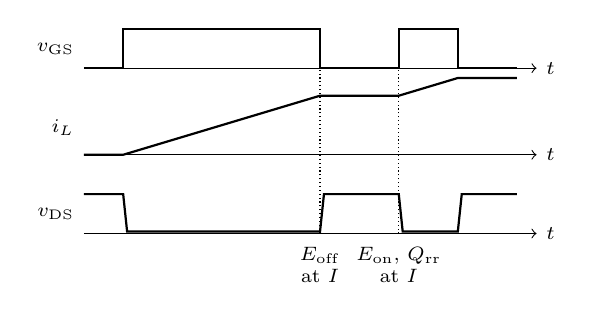
\begin{tikzpicture}[x=0.5cm, y=0.5cm, font=\scriptsize]
					% gate signal
					\draw[->] (0,4.2) -- (11.5,4.2) node[right] {$t$};
					\draw[thick] (0,4.2) -- (1,4.2) -- (1,5.2) -- (6,5.2) -- (6,4.2) -- (8,4.2) -- (8,5.2) -- (9.5,5.2) -- (9.5,4.2) -- (11,4.2);
					\node[anchor=east] at (0,4.7) {$v_\mathrm{GS}$};
					% inductor current
					\draw[->] (0,2.0) -- (11.5,2.0) node[right] {$t$};
					\draw[thick] (0,2.0) -- (1,2.0) -- (6,3.5) -- (8,3.5) -- (9.5,3.95) -- (11,3.95);
					\node[anchor=east] at (0,2.7) {$i_L$};
					% drain-source voltage
					\draw[->] (0,0) -- (11.5,0) node[right] {$t$};
					\draw[thick] (0,1.0) -- (1,1.0) -- (1.1,0.05) -- (6,0.05) -- (6.1,1.0) -- (8,1.0) -- (8.1,0.05) -- (9.5,0.05) -- (9.6,1.0) -- (11,1.0);
					\node[anchor=east] at (0,0.5) {$v_\mathrm{DS}$};
					\draw[densely dotted] (6,0) -- (6,5.2) (8,0) -- (8,5.2);
					\node[anchor=north, align=center] at (6,-0.1) {$E_\mathrm{off}$\\at $I$};
					\node[anchor=north, align=center] at (8,-0.1) {$E_\mathrm{on}$, $Q_\mathrm{rr}$\\at $I$};
				\end{tikzpicture}
				\caption{Pulse 1 builds up $I=V_\mathrm{DC}t_1/L$; the edges at its end and at the start of pulse 2 are measured}
			\end{figure}
		\end{column}
	\end{columns}
	\small
	The pulses last only microseconds: the junction stays at the heat-sink temperature, and every operating point ($V$, $I$, $T$, $R_\mathrm{G}$) can be set independently.
	\blfootnote{Source: Wang, Zhang, Jones, 2018, Ch.\ 4.}
\end{frame}

%%%%%%%%%%%%%%%%%%%%%%%%%%%%%%%%%%%%%%%%%%%%%%%%%%%%%%%%%%%%%
%% DPT pitfalls %%
%%%%%%%%%%%%%%%%%%%%%%%%%%%%%%%%%%%%%%%%%%%%%%%%%%%%%%%%%%%%%
\begin{frame}
	\frametitle{Reading double-pulse results}
	\begin{columns}[T]
		\begin{column}{0.5\textwidth}
			\small
			\textbf{Where the energy goes}
			\begin{itemize}
				\item Measured at the terminals, $E_\mathrm{off}$ contains the energy $E_\mathrm{oss}$ that charges $C_\mathrm{oss}$ of the DUT; it is not lost yet.
				\item At the next turn-on $C_\mathrm{oss}$ discharges inside the DUT, through its channel. The terminals do not see this current: the measured $E_\mathrm{on}$ is too small by $E_\mathrm{oss}$.
				\item The sum $E_\mathrm{on}+E_\mathrm{off}$ is right; the split is not. Correction with the turn-off energy measured at zero current: $E_\mathrm{on}+E_\mathrm{off,0A}$ and $E_\mathrm{off}-E_\mathrm{off,0A}$.
			\end{itemize}
		\end{column}
		\begin{column}{0.47\textwidth}
			\small
			\textbf{What a double-pulse test cannot show}
			\begin{itemize}
				\item Loss under ZVS: $C_\mathrm{oss}$ hysteresis and the partial charge of a soft transition
				\item Dynamic $R_\mathrm{DS(on)}$ in continuous operation and its thermal steady state
				\item The parasitics of your own layout: the test board has its own loop
			\end{itemize}
			\textbf{Pitfalls}: skew, bandwidth, probe loading, insertion inductance of the shunt, ringing counted into the edge.
		\end{column}
	\end{columns}
	\blfootnote{Source: Wang, Zhang, Jones, 2018, Sec.\ 3.8 and 8.10.}
\end{frame}

%%%%%%%%%%%%%%%%%%%%%%%%%%%%%%%%%%%%%%%%%%%%%%%%%%%%%%%%%%%%%
%% Soft-switching loss %%
%%%%%%%%%%%%%%%%%%%%%%%%%%%%%%%%%%%%%%%%%%%%%%%%%%%%%%%%%%%%%
\begin{frame}
	\frametitle{Measuring $C_\mathrm{oss}$ loss}
	\begin{columns}[T]
		\begin{column}{0.42\textwidth}
			\begin{figure}
				\centering
				\begin{circuitikz}[scale=0.68, transform shape]
					\draw (0,0) node[ground]{} to[sV, l=RF amplifier] (0,3.2) to[L, l=$L_\mathrm{r}$] (2.4,3.2) coordinate (y);
					\draw (y) node[circ]{} node[above]{$v_\mathrm{Y}$} to[C, l=DUT $C_\mathrm{oss}$] (2.4,1.4) coordinate (x);
					\draw (x) node[circ]{} to[C, l=$C_\mathrm{ref}$] (2.4,0) node[ground]{};
					\draw (x) -- (3.4,1.4) node[right]{$v_\mathrm{X}$};
				\end{circuitikz}
				\caption{Sawyer--Tower circuit (simplified)}
			\end{figure}
			\small
			$Q_\mathrm{oss}=C_\mathrm{ref}v_\mathrm{X}$, $v_\mathrm{DS}=v_\mathrm{Y}-v_\mathrm{X}$:
			\begin{equation*}
				E_\mathrm{diss}=\oint v_\mathrm{DS}\,\mathrm{d}Q_\mathrm{oss}
			\end{equation*}
		\end{column}
		\begin{column}{0.55\textwidth}
			\small
			\begin{itemize}
				\item The area of the $Q$--$V$ loop is the energy lost per cycle (L2). Zulauf et al.: sub-$\mu$J resolution at 650\,V and up to 35\,MHz; skew between $v_\mathrm{X}$ and $v_\mathrm{Y}$ calibrated; cross-check by the temperature rise (infrared camera).
				\item Sine excitation is not the converter waveform; losses rise with $\mathrm{d}v/\mathrm{d}t$.
				\item Calorimetric alternative: active and passive half-bridge on a resonant tank, so the DUT sees the real square-wave $v_\mathrm{DS}$; the loss follows from the calibrated temperature rise. A calibration without thermal equilibrium cuts the time per point from over an hour to below one minute.
				\item Small-signal $C$--$V$ curves (impedance analyser and bias tee) show no hysteresis.
			\end{itemize}
		\end{column}
	\end{columns}
	\blfootnote{Sources: Zulauf et al., IEEE TPEL, vol.\ 33, no.\ 12, 2018; de Filippis and Kasper, How2Power Today, May 2024.}
\end{frame}

%%%%%%%%%%%%%%%%%%%%%%%%%%%%%%%%%%%%%%%%%%%%%%%%%%%%%%%%%%%%%
%% Dynamic R_DS(on) %%
%%%%%%%%%%%%%%%%%%%%%%%%%%%%%%%%%%%%%%%%%%%%%%%%%%%%%%%%%%%%%
\begin{frame}
	\frametitle{Dynamic on-resistance}
	\begin{columns}[T]
		\begin{column}{0.5\textwidth}
			\small
			$R_\mathrm{DS(on)}$ right after turn-on needs $v_\mathrm{DS}$ with mV resolution, while the same channel saw 400\,V a moment earlier.
			\begin{itemize}
				\item About 9 effective bits: on a 400\,V range one step is 0.78\,V.
				\item A sensitive range overdrives the input amplifier during the off-state; it needs time to recover.
			\end{itemize}
			A clamp circuit at the DUT limits the voltage seen by the scope to a few volts. The scope can then use a fine range; valid on-state data within about 100\,ns after turn-on.
		\end{column}
		\begin{column}{0.47\textwidth}
			\small
			\begin{itemize}
				\item Measure in double-pulse or in continuous operation at the stress of the application (voltage, off-time, temperature, frequency).
				\item Report $R_\mathrm{DS(on)}$ versus time after turn-on.
				\item Test method guidelines: JEDEC JEP173 (2019).
				\item At MHz the conduction time is short: the dynamic value is the one that counts (L2).
			\end{itemize}
		\end{column}
	\end{columns}
	\blfootnote{Sources: Arai et al., Dynamic on-resistance measurement techniques for GaN power transistors, Bodo's Power Systems, reprinted by EEPower; JEDEC JEP173, 2019.}
\end{frame}

%%%%%%%%%%%%%%%%%%%%%%%%%%%%%%%%%%%%%%%%%%%%%%%%%%%%%%%%%%%%%
%% Impedance measurement %%
%%%%%%%%%%%%%%%%%%%%%%%%%%%%%%%%%%%%%%%%%%%%%%%%%%%%%%%%%%%%%
\subsection{Passive components}

\begin{frame}
	\frametitle{Impedance measurement}
	\begin{columns}[T]
		\begin{column}{0.5\textwidth}
			\begin{table}
				\centering
				\footnotesize
				\begin{tabular}{|l|>{\raggedright\arraybackslash}p{3.4cm}|}
					\hline
					\textbf{Method}            & \textbf{Range of about 10\,\% accuracy}            \\
					\hline
					auto-balancing bridge      & m$\Omega$ to 100\,M$\Omega$, up to about 100\,MHz   \\
					VNA reflection ($S_{11}$)  & about 1\,$\Omega$ to 2\,k$\Omega$                  \\
					VNA series-through         & about 5\,$\Omega$ to 20\,k$\Omega$                 \\
					VNA shunt-through ($S_{21}$) & 1\,m$\Omega$ to 5\,$\Omega$                     \\
					\hline
				\end{tabular}
				\caption{Impedance ranges (Keysight)}
			\end{table}
			\small
			Shunt-through, $Z_0=50\,\Omega$: $Z=25\,\Omega\cdot S_{21}/(1-S_{21})$.
		\end{column}
		\begin{column}{0.47\textwidth}
			\small
			\begin{itemize}
				\item Reflection fails at m$\Omega$: for 5\,m$\Omega$, $\Gamma=-0.9998$; an error of 0.1\,\% in $|\Gamma|$ turns the result into $-20$\,m$\Omega$.
				\item Fixture compensation: open, short and load measured in the fixture remove its parasitics.
				\item Below about 100\,kHz the ground loop between the two ports of the VNA spoils shunt-through results: use an isolating receiver or a common-mode choke.
				\item Measure at the operating condition: DC bias, temperature and AC level change ceramics and ferrites.
			\end{itemize}
		\end{column}
	\end{columns}
	\blfootnote{Sources: Keysight, Impedance Measurement Handbook; Keysight, Performing Impedance Analysis with the E5061B ENA, 2024.}
\end{frame}

%%%%%%%%%%%%%%%%%%%%%%%%%%%%%%%%%%%%%%%%%%%%%%%%%%%%%%%%%%%%%
%% Capacitor model %%
%%%%%%%%%%%%%%%%%%%%%%%%%%%%%%%%%%%%%%%%%%%%%%%%%%%%%%%%%%%%%
\begin{frame}
	\frametitle{Capacitor model from $|Z(f)|$}
	\begin{columns}[T]
		\begin{column}{0.52\textwidth}
			\begin{figure}
				\centering
				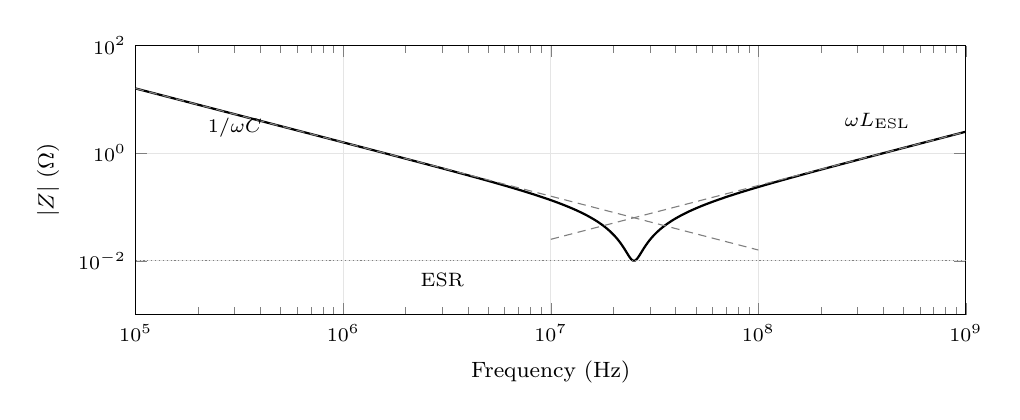
\begin{tikzpicture}
					\begin{axis}[
							width=\linewidth, height=5.0cm,
							xmode=log, ymode=log, xmin=1e5, xmax=1e9, ymin=1e-3, ymax=100,
							xlabel={Frequency (Hz)}, ylabel={$|Z|$ ($\Omega$)},
							grid=major, grid style={gray!20},
							tick label style={font=\scriptsize}, label style={font=\footnotesize},
						]
						\addplot[black, thick, domain=5:9, samples=400] ({10^x}, {sqrt(0.01^2+(2*pi*10^x*0.4e-9-1/(2*pi*10^x*100e-9))^2)});
						\addplot[gray, densely dashed, domain=5:8, samples=2] ({10^x}, {1/(2*pi*10^x*100e-9)});
						\addplot[gray, densely dashed, domain=7:9, samples=2] ({10^x}, {2*pi*10^x*0.4e-9});
						\addplot[gray, densely dotted, domain=5:9, samples=2] ({10^x}, {0.01});
						\node[font=\scriptsize, anchor=west] at (axis cs:2e5,3) {$1/\omega C$};
						\node[font=\scriptsize, anchor=east] at (axis cs:6e8,4) {$\omega L_\mathrm{ESL}$};
						\node[font=\scriptsize, anchor=north] at (axis cs:3e6,0.009) {ESR};
					\end{axis}
				\end{tikzpicture}
				\caption{100\,nF, ESR 10\,m$\Omega$, ESL 0.4\,nH: self-resonance at 25\,MHz}
			\end{figure}
		\end{column}
		\begin{column}{0.45\textwidth}
			\small
			Fit a series $R$--$L$--$C$ to the measured $|Z|$ and phase:
			\begin{itemize}
				\item $C$ from the capacitive slope, $L_\mathrm{ESL}$ from the inductive slope
				\item ESR at the minimum, $f_\mathrm{SRF}=1/(2\pi\sqrt{L_\mathrm{ESL}C})$
			\end{itemize}
			The ESL depends on the mounting: pads, vias and the distance to the plane (L3). Measure the capacitor on a fixture that resembles the board, or the board itself.\\[0.4em]
			Above $f_\mathrm{SRF}$ the part is an inductor. Several values in parallel create anti-resonances (L3).
		\end{column}
	\end{columns}
\end{frame}

%%%%%%%%%%%%%%%%%%%%%%%%%%%%%%%%%%%%%%%%%%%%%%%%%%%%%%%%%%%%%
%% Magnetics %%
%%%%%%%%%%%%%%%%%%%%%%%%%%%%%%%%%%%%%%%%%%%%%%%%%%%%%%%%%%%%%
\begin{frame}
	\frametitle{Core loss at MHz}
	\begin{columns}[T]
		\begin{column}{0.5\textwidth}
			\small
			\textbf{Two-winding method}: $P=\frac{1}{T}\int v_2\,i_1\,\mathrm{d}t\cdot\frac{N_1}{N_2}$ excludes the copper loss of the drive winding. For a low-loss core $v$ and $i$ are almost $90^\circ$ apart:
			\begin{equation*}
				\frac{\Delta P}{P}\approx Q\,\Delta\varphi
			\end{equation*}
			10\,MHz, 100\,ps skew: $\Delta\varphi=0.36^\circ$. With $Q=100$ the loss is wrong by 63\,\%.
		\end{column}
		\begin{column}{0.47\textwidth}
			\small
			\textbf{Resonant methods}
			\begin{itemize}
				\item A capacitor cancels the reactive voltage; the phase sensitivity drops.
				\item Resonant $Q$ method: series tank driven at resonance, $Q=V_\mathrm{out}/V_\mathrm{in}$, no phase measurement:
				      \begin{equation*}
					      R_\mathrm{core}=\frac{2\pi fL\,V_\mathrm{in}}{V_\mathrm{out}}-R_\mathrm{C}-R_\mathrm{cu}
				      \end{equation*}
				      accurate to better than 20\,\%.
				\item A DC bias can raise the core loss of NiZn ferrite at 10\,MHz by a factor of three: measure with bias.
			\end{itemize}
		\end{column}
	\end{columns}
	\blfootnote{Sources: Han et al., IEEE TPEL, vol.\ 27, no.\ 1, 2012; Hanson et al., IEEE TPEL, vol.\ 31, no.\ 11, 2016, App.\ B and C.}
\end{frame}

%%%%%%%%%%%%%%%%%%%%%%%%%%%%%%%%%%%%%%%%%%%%%%%%%%%%%%%%%%%%%
%% Efficiency and temperature %%
%%%%%%%%%%%%%%%%%%%%%%%%%%%%%%%%%%%%%%%%%%%%%%%%%%%%%%%%%%%%%
\subsection{Efficiency and temperature}

% Two pages: task (page 1) and task with solution (page 2).
\begin{frame}<handout:1-2>
	\frametitle{Loss from efficiency}
	\begin{block}{Task (4 minutes)}
		A converter takes 100\,W and delivers 98\,W. Input and output power are measured with an accuracy of $\pm0.1\,\%$ of reading each.
		\begin{enumerate}
			\item How accurate is the loss?
			\item Repeat for 99\,\% efficiency.
			\item Which accuracy per reading gives $\pm5\,\%$ of the loss at 99\,\%?
		\end{enumerate}
	\end{block}
	\onslide<2-|handout:2>{
		\begin{enumerate}
			\item $P_\mathrm{loss}=2$\,W; worst case $\pm(0.1+0.098)$\,W $=\pm0.198$\,W, i.e.\ $\pm9.9\,\%$ ($\pm7\,\%$ if the two errors are independent).
			\item $P_\mathrm{loss}=1$\,W, $\pm0.199$\,W: $\pm20\,\%$. The error grows with $1/(1-\eta)$.
			\item $\pm0.05\,\mathrm{W}/199\,\mathrm{W}=\pm0.025\,\%$ per reading, and the sensors must keep it up to the switching frequency.
		\end{enumerate}
		{\small At high efficiency a direct measurement of the loss (calorimetry) is more accurate than a difference of two large numbers.}
	}
\end{frame}

%%%%%%%%%%%%%%%%%%%%%%%%%%%%%%%%%%%%%%%%%%%%%%%%%%%%%%%%%%%%%
%% Calorimetry and temperature %%
%%%%%%%%%%%%%%%%%%%%%%%%%%%%%%%%%%%%%%%%%%%%%%%%%%%%%%%%%%%%%
\begin{frame}
	\frametitle{Calorimetry and temperature}
	\begin{columns}[T]
		\begin{column}{0.5\textwidth}
			\small
			\textbf{Calorimetric loss measurement}
			\begin{itemize}
				\item The heat leaving a closed chamber (heat flux through the walls or coolant flow and temperature rise) gives the loss directly.
				\item Calibration with a known DC power in the same chamber.
				\item Accuracy does not depend on the efficiency, but each operating point takes from minutes to hours.
			\end{itemize}
		\end{column}
		\begin{column}{0.47\textwidth}
			\small
			\textbf{Temperature at MHz}
			\begin{itemize}
				\item Infrared camera: shiny metal has an emissivity of 0.1 or less, the camera is accurate above about 0.7. Matte tape or paint on the part. Example: a metal package read 27.5\,$^\circ$C bare and 43.9\,$^\circ$C with polyimide tape, i.e.\ 87\,\% of the temperature rise was missed.
				\item Thermocouples in strong HF fields pick up voltages and can be heated by eddy currents; fibre-optic sensors avoid both.
				\item Thermal cross-coupling between neighbouring parts blurs the loss of each part (Zulauf et al.).
			\end{itemize}
		\end{column}
	\end{columns}
	\blfootnote{Sources: Christen, Badstuebner, Biela, Kolar, IPEC 2010; Lidow et al., 2019, Sec.\ 6.4.4; Zulauf et al., 2018.}
\end{frame}

%%%%%%%%%%%%%%%%%%%%%%%%%%%%%%%%%%%%%%%%%%%%%%%%%%%%%%%%%%%%%
%% Key messages %%
%%%%%%%%%%%%%%%%%%%%%%%%%%%%%%%%%%%%%%%%%%%%%%%%%%%%%%%%%%%%%
\begin{frame}
	\frametitle{Key messages}
	\begin{enumerate}
		\item Probe and scope must be about four times faster than the edge; rise times add geometrically.
		\item A ground lead of a few cm rings at a few hundred MHz: spring tip or coaxial test point. A ring that changes with the probing is an artefact.
		\item High-side $v_\mathrm{GS}$ needs an optically isolated probe; a differential probe has only about 30\,dB CMRR at 100\,MHz.
		\item A shunt measures $Ri+L_\mathrm{s}\,\mathrm{d}i/\mathrm{d}t$; at 10\,m$\Omega$ even 10\,pH matter. Plan current sensing with the layout.
		\item One nanosecond of skew can double or erase the measured switching energy. Deskew, and check the result against a physical marker.
		\item Double-pulse tests give the sum $E_\mathrm{on}+E_\mathrm{off}$, not ZVS losses. $C_\mathrm{oss}$ loss and core loss at MHz need dedicated methods.
	\end{enumerate}
\end{frame}

%%%%%%%%%%%%%%%%%%%%%%%%%%%%%%%%%%%%%%%%%%%%%%%%%%%%%%%%%%%%%
%% Exit ticket %%
%%%%%%%%%%%%%%%%%%%%%%%%%%%%%%%%%%%%%%%%%%%%%%%%%%%%%%%%%%%%%
% Two pages: questions (page 1) and answers (page 2).
\begin{frame}<handout:1-2>
	\frametitle{Exit questions}
	\begin{varblock}[\textwidth]{Three questions, one minute each}
		\begin{enumerate}
			\item Your scope shows ringing at 180\,MHz on the switch node. How do you find out whether it is real?
			\item Why does the measured $E_\mathrm{on}$ of a double-pulse test underestimate the loss of a hard turn-on, even with perfect probes?
			\item A core is measured with the two-winding method at 5\,MHz, $Q=50$. Which skew between voltage and current gives 10\,\% error in the loss?
		\end{enumerate}
	\end{varblock}
	\onslide<2-|handout:2>{
		\begin{enumerate}
			\item Change the probing (spring tip, coaxial test point) and compare with $1/(2\pi\sqrt{L_\mathrm{loop}C})$. A ring that moves with the probing is an artefact.
			\item The $C_\mathrm{oss}$ of the DUT discharges inside the device; the terminals do not see this current. The energy appears in the measured $E_\mathrm{off}$ instead.
			\item $\Delta\varphi=0.1/50=2\,\mathrm{mrad}=0.115^\circ$; $\Delta t=\Delta\varphi/(2\pi f)=64$\,ps.
		\end{enumerate}
	}
\end{frame}

%%%%%%%%%%%%%%%%%%%%%%%%%%%%%%%%%%%%%%%%%%%%%%%%%%%%%%%%%%%%%
%% References %%
%%%%%%%%%%%%%%%%%%%%%%%%%%%%%%%%%%%%%%%%%%%%%%%%%%%%%%%%%%%%%
\begin{frame}
	\frametitle{References}
	\scriptsize
	\begin{itemize}
		\item F. Wang, Z. Zhang, E.\,A. Jones, \textit{Characterization of Wide Bandgap Power Semiconductor Devices}, IET, 2018.
		\item Keysight, \textit{Evaluating Oscilloscope Bandwidths for Your Application}, application note 5989-5733EN, 2019; \textit{Impedance Measurement Handbook}; \textit{Performing Impedance Analysis with the E5061B ENA Vector Network Analyzer}, 2024.
		\item ROHM, \textit{Method for Monitoring Switching Waveform}, application note.
		\item L. Shillaber, Y. Jiang, L. Ran, T. Long, ``Ultra fast current shunt (UFCS): a gigahertz bandwidth ultra low inductance current sensor,'' IEEE Trans.\ Power Electron., 2022.
		\item G. Zulauf, S. Park, W. Liang, K.\,N. Surakitbovorn, J. Rivas-Davila, ``$C_\mathrm{OSS}$ losses in 600\,V GaN power semiconductors in soft-switched, high- and very-high-frequency power converters,'' IEEE Trans.\ Power Electron., vol.\ 33, no.\ 12, pp.\ 10748--10763, 2018.
		\item S. de Filippis, M.\,J. Kasper, ``Characterizing dynamic $C_\mathrm{OSS}$ losses in 600-V GaN HEMTs,'' How2Power Today, May 2024.
		\item T. Arai et al., ``Dynamic on-resistance measurement techniques for GaN power transistors,'' Bodo's Power Systems; JEDEC JEP173, \textit{Dynamic On-Resistance Test Method Guidelines for GaN HEMT Based Power Conversion Devices}, 2019.
		\item Y. Han, G. Cheung, A. Li, C.\,R. Sullivan, D.\,J. Perreault, ``Evaluation of magnetic materials for very high frequency applications,'' IEEE Trans.\ Power Electron., vol.\ 27, no.\ 1, pp.\ 425--435, 2012.
		\item A.\,J. Hanson, J.\,A. Belk, S. Lim, C.\,R. Sullivan, D.\,J. Perreault, ``Measurements and performance factor comparisons of magnetic materials at high frequency,'' IEEE Trans.\ Power Electron., vol.\ 31, no.\ 11, pp.\ 7909--7925, 2016.
		\item D. Christen, U. Badstuebner, J. Biela, J.\,W. Kolar, ``Calorimetric power loss measurement for highly efficient converters,'' IPEC 2010, pp.\ 1438--1445.
	\end{itemize}
\end{frame}
